\documentclass{article}
\usepackage[margin=1in]{geometry} 
\usepackage{amsmath,amsthm,amssymb,amsfonts, fancyhdr, color, comment, graphicx, environ}
\usepackage{xcolor}
\usepackage{mdframed}
\usepackage[shortlabels]{enumitem}
\usepackage{indentfirst}
\usepackage{hyperref}
\hypersetup{
    colorlinks=true,
    linkcolor=blue,
    filecolor=magenta,      
    urlcolor=blue,
}
\usepackage{pgfplots}
\pgfplotsset{width=10cm,compat=1.9}
\pgfplotsset{compat=1.17}
\usepackage{tikz}
\usepackage{caption}

\setlength{\parindent}{0pt}


%for headers 
\pagestyle{fancy}
\fancyhf{} % for header/footer

\lhead{Creel}
\rhead{ENV 795 - Nature as Capital}
\chead{\textbf{Dynamic Concepts}}

\title{Week Three - Dynamic Concepts}
\author{Andie Creel for Nature as Capital}
\date{February 13th, 2023}


\begin{document}
\maketitle

\section{Utility}
\begin{itemize}
    \item Utility does not have units. It is ordinal (not cardinal), it's just a ranking. Ex. A is better than B, but we cannot say A is two times better than B. 
    \item We also must make trade offs. Given the choices and the constraints, you want to choose the option without violating your constraints. 
    \item Example of contour map: you want to go up the mountain as far as you can without losing oxygen. 
\end{itemize}

\begin{figure}[htp]
    \centering
    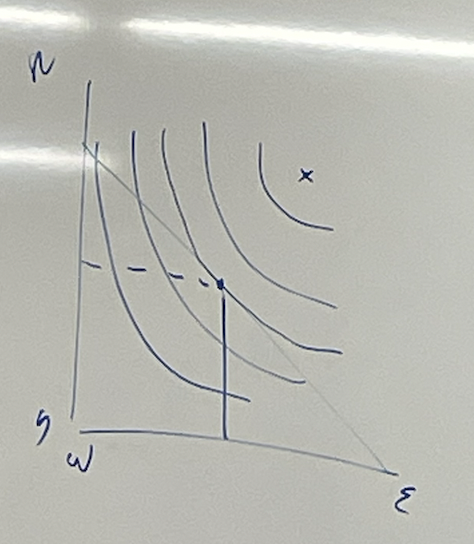
\includegraphics[width=7cm]{contour_map.png}
    \caption{Contour Map}
\end{figure}

We often model utility \textit{functions} with \textbf{logs}:
$$U(X,Y)  = X^\alpha Y^\beta$$
A log transformation of the above utility function is (this is just following log rules):
$$ln(U) = \alpha * ln(X) + \beta * ln(Y)$$

\section{Utility Across Time}
\begin{itemize}
    \item Generally: Would you prefer something today or something tomorrow?
    \item Would you give Eli \$10 today if he was guaranteed to give it back to you tomorrow? No, because you prefer \$10 today more than \$10 a year from now. 
    \item We cannot compare utility across \textit{individuals} but we can compare one individual's utility across time. However, we need to discount the future because we prefer utility sooner rather than later. 
    Consider two time periods
    $$U_0 + \beta U_1$$
    where $\beta$ is the discount factor and $0<\beta<1$.
    \item Consider three time periods:
     $$U_0 + \beta U_1 + \beta \beta U_2 =  \beta ^ 0U_0 + \beta^1 U_1 + \beta^2 U_2 $$
     \item Discount factor in continuous time: $\beta^t = e^{-rt}$
     \item Discount factor in discrete time : $\beta^t = (\frac{1}{1+r})^t$
     
\end{itemize}

\section{Discounting and Climate Change}
\begin{itemize}
    \item When we calculate the social cost of carbon, we must choose a discount rate (how much we value the future). 
    \item The choice of the discount rate leads to REALLY different SCC! 
    \item Two main people in the discount rate debate: Nick Stern (wants a really low discount rate which leads to a higher SCC) and Bill Nordhaus (wants a higher discount rate which leads to a lower SCC). 
    \item Ramsey Rule (1928): The core economic theory for discounting 
    $$r(g) = \rho + \eta g$$
    where $r$ is the social discount rate or consumptive discount rate, $\rho$ is the utility discount rate, $\eta$ is the consumption elasticity of marginal utility and $g$ is the growth rate.
    \item Importance of using a discount rate: If you're using a 7\% discount rate and are considering doing a project that won't provide benefits until 30 years from now, this high discount rate means that the discounted benefits won't be greater than the costs incurred today.
    \item Nordhaus went from 3\% to 1.5\%... why? Empirical evidence. When you look at US treasury bonds, we see that the U.S. governments bonds following a 1.5\% discount rate in more recent years. This is different! In the 70s, it had been up near 3\%. Why is this happening? Modern monetary economics doesn't have a clear answer year. BUT a major point may be rising inequality (Bauer and Rudebusch 2021). 
    \item Sustainable development focuses on inter-temporal inequality. But we also should be concerned of equity within this current generation. 
    
\end{itemize}

\section{Summing utility functions}
Let's say your utility in every time period is $v$, $u_t = v$. You want to sum your own utility over multiple years to get your welfare function, 

$$ Benefits = \int_0^T exp(-rt) v dt + S(T)$$

$$ Benefits = \int_0^\infty exp(-rt)vdt = - \frac{v}{r}exp(-rt)|_0^\infty = \frac{v}{r}$$

Note that in both of these cases we are only summing ONE persons utility through time. We are not aggregating across people. 

\section{Negishi Weights}
Summing across people. Negishi weights rely on the inverse marginal utility of income, $\eta$.  The more your willing to give up for something, the higher weight you have. Well, what happens then if I'm poor and you're rich? I'm only willing to give up \$5 but you're willing to give up \$500 because you're rich. \\

Negishi weight: $\alpha = \frac{1}{\eta}$\\

Consider the utility function 
$$U(C) = \frac{C^{1-\eta} - 1}{1 - \eta}$$

\begin{figure}[htp]
    \centering
    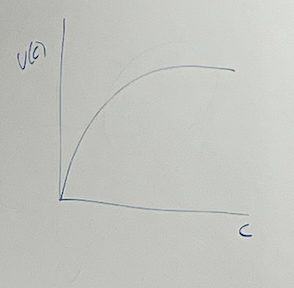
\includegraphics[width=7cm]{Screen Shot 2023-02-13 at 10.12.33 AM.png}
    \caption{Utility function}
\end{figure}

If you're consuming a lot, your marginal utility is 0. So the inverse of that is $\infty$. And so you're Negishi weight is HUGE and you get a huge Negishi weight, and if we were to add your utility to another, we'd give it a huge weight. 


\section{Review of Ramsey Rule}

$$r(g) = \rho + \eta g$$

where $g = \frac{\dot w}{w}$ and is the growth rate of monetary capital (consumption opportunities). It's a growth rate because it's the change divided by the level. You can't hand someone utility, but you can hand them assets that provide utility. So we can measure our wealth as capital assets. \\

Consider adding natural capital that is not fungible with monetary capital 
$$r = \rho + \eta \frac{\dot w}{w} + \psi \frac{\dot s}{s}$$
the Ramsey rule is now going to consider the growth (or decline) of natural capital.\\

\subsection{Risk-Certainty Equivalence}
If you have a utility function that looks like figure 2, your preference is to avoid risk. \\

Consider the utility function 
$$ U(C) = \frac{C^{1-\eta} - 1}{1 - \eta}.$$
Note that marginal utility is 
$$\frac{\partial U}{\partial C} =U'(C) = C^{-\eta}.$$

\begin{figure}[htp]
    \centering
    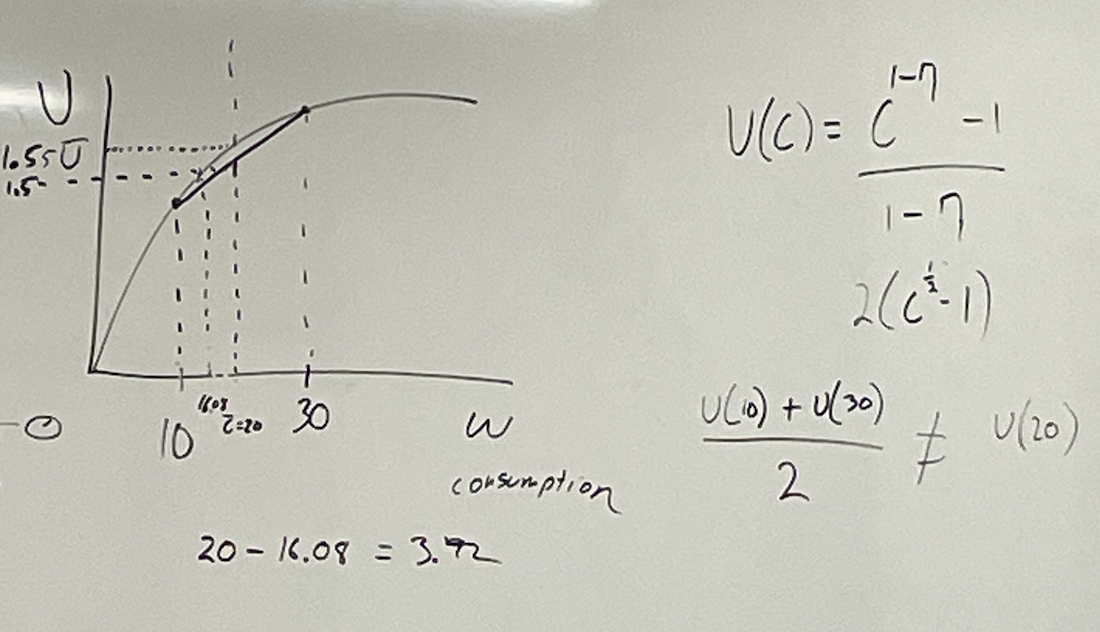
\includegraphics[width=12cm]{Screen Shot 2023-02-15 at 9.24.07 AM.png}
    \caption{Utility function}
\end{figure}

Because of the curvature of utility, 
$$\frac{U(10) + U(30)}{2} < U(20).$$

If utility was linear, these would be equivalent! But utility is concave. \\

Let the utility function be 
$$ U(C) = \frac{C^{1-1/2} - 1}{1 - 1/2}$$
$$= 2(C^{\frac{1}{2}} - 1).$$

What the Risk-Certainty Equivalence says is I would be indifferent between having 16.08 ( $=  \frac{U(10) + U(30)}{2}$) units of consumption GUARANTEED and a lottery where there is a 50\% I get 10 units of consumption and a 50\% chance I get 30 units of consumption. When you don't like risk (i.e., your utility function is concave) then you'd accept some a certain level of consumption guaranteed that is slightly less than the expected units of consumption from a lottery. 

\end{document}
